% =====================================================================
%  LabSteward -- IEEE conference draft (ICEIB 2027 target)
%  Template : IEEEtran (conference)   Compiler: pdfLaTeX on Overleaf
%  Rules    : English, 4--8 pages, every body paragraph carries a
%             "% [A2Z:<code>]" tag (checked by check_a2z.py).
%  Numbers  : every figure in Sec. IV is traceable to
%             ../experiments/results_real_eval*.json. Anything that has
%             not been measured is written as \TBD.
%  OpenSpec : each section is governed by openspec/changes/00N_*.
% =====================================================================
\documentclass[conference]{IEEEtran}
\IEEEoverridecommandlockouts
\usepackage{cite}
\usepackage{amsmath,amssymb,amsfonts}
\usepackage{algorithmic}
\usepackage{algorithm}
\usepackage{graphicx}
\usepackage{textcomp}
\usepackage{booktabs}
\usepackage{multirow}
\usepackage{array}
\usepackage{xcolor}
\usepackage{tikz}
\usetikzlibrary{arrows.meta,positioning,fit,calc}
\usepackage{url}
\newcommand{\TBD}{\textcolor{red}{[TBD]}}
\def\BibTeX{{\rm B\kern-.05em{\sc i\kern-.025em b}\kern-.08em
    T\kern-.1667em\lower.7ex\hbox{E}\kern-.125emX}}

\begin{document}

\title{Utilize Before Acquire: A Guardrailed Tool-Calling Agent for
University Laboratory Asset Lifecycle Management and Public-Procurement
Compliance\\
{\footnotesize Draft for ICEIB 2027 --- results measured on a 50-task benchmark}}

\author{
\IEEEauthorblockN{Author Name 1, Author Name 2, Author Name 3, Author Name 4, Author Name 5}
\IEEEauthorblockA{\textit{Dept. of Computer Science and Engineering} \\
\textit{National Chung Hsing University}\\
Taichung, Taiwan \\
zhaobin2638@gmail.com}
}

\maketitle

% ---------------------------------------------------------------------
\begin{abstract}
% [A2Z:A]
Universities spend large public budgets on research instruments, yet
many devices sit idle while laboratories keep buying new ones.
% [A2Z:B]
Campus systems only record ownership, not use; general LLM agents are
unstable on multi-step tool tasks and know nothing about procurement
thresholds or statutory service lives.
% [A2Z:C]
We present LabSteward, an agent that enforces a \emph{utilize before
acquire} rule: every purchase request is first matched against idle
inventory.
% [A2Z:D]
A planner routes requests to management and procurement sub-agents,
while all numbers, state transitions and threshold decisions are made by
deterministic tools, a dual-track (book vs.\ market) residual-value model
and a YAML rule guardrail.
% [A2Z:E]
We executed the released code on a 50-task benchmark (25 management, 25
procurement) under two state protocols and repeated runs, and measured
every outcome instead of reusing the hard-coded figures of an earlier
evaluation script.
% [A2Z:F]
The released version solves 40.0\% of tasks (60.0\% management, 20.0\%
procurement); two one-line fixes raise this to 60.0\% with 100\%
management success. The idle-inventory pre-check caught all repeated
purchase requests, and no guardrail-blocked task reached a successful
outcome, but one disposal path was stopped only by a crash. Procurement
remains limited by catalogue coverage and by running the guardrail after
vendor search.
\end{abstract}

\begin{IEEEkeywords}
LLM agent, tool calling, guardrail, asset management, public procurement,
residual value, spec-driven development
\end{IEEEkeywords}

% =====================================================================
\section{Introduction}
% ---------------------------------------------------------------------
% [A2Z:G]
Research equipment is one of the largest capital items in a university
budget, and the rise of GPU-based AI research has made individual
purchases more expensive than ever. At the same time, procurement is
moving toward agentic automation, where software agents search vendors,
compare offers and draft requests with little human
effort~\cite{yao2023react,singh2025agenticrag}.

% [A2Z:H]
Three gaps remain. First, utilization is invisible: Taiwan's Control
Yuan found expensive instruments funded by national grants left unused
for long periods~\cite{controlyuan2013}, because campus property systems
record who owns an asset but not whether it is used. Second, LLM agents
are unreliable on long tool-calling tasks: on $\tau$-bench, even strong
models succeed on all eight repeated trials of the same retail task less
than 25\% of the time~\cite{yao2024taubench}, and shopping agents
mis-filter products~\cite{lyu2025deepshop}. Third, public procurement is
rule-bound: the Government Procurement Act defines small-purchase and
announcement thresholds and forbids splitting one need into several
orders to stay under them~\cite{gpa_tw}, while accounting service lives
rarely match the real economic life of an instrument~\cite{huymajer2025residual}.

% [A2Z:I]
Prior solutions evolved in four steps: (1) relational property ledgers
with straight-line depreciation; (2) machine-learning residual-value and
entity-matching models~\cite{huymajer2025residual,peeters2025entity};
(3) end-to-end LLM agents that call tools through
reasoning traces~\cite{yao2023react,schick2023toolformer}; and (4)
hybrid designs in which an LLM coordinates while solvers or retrieval
modules produce the answers~\cite{duan2025askclarify,singh2025agenticrag}.

% [A2Z:J]
Ledgers are auditable but passive; ML valuers are accurate but blind to
law; end-to-end agents are flexible but unstable and can state wrong
thresholds; hybrid designs are promising but have not been applied to
the full asset lifecycle together with procurement law. None of them
checks idle inventory before buying.

% [A2Z:K]
Our key idea is to make \emph{utilize before acquire} a hard step of the
procurement flow, and to move every number and every legal decision out
of the language model. Our contributions are: (i) the LabSteward
architecture with two domain sub-agents, deterministic tools and an
external rule guardrail; (ii) a dual-track residual-value model that
reports both statutory book value and an interval for market value;
(iii) an OpenSpec-governed, open-source implementation; and (iv) a
measured evaluation that reports failures as well as successes,
including two defects found by the measurement itself.

% [A2Z:L]
Section~II reviews related work, Section~III presents the design,
Section~IV reports the experiments, and Section~V concludes.

% =====================================================================
\section{Related Work}
% ---------------------------------------------------------------------
% [A2Z:M]
\textit{Accounting and econometric baselines.} Government property rules
depreciate assets on a straight line over a statutory minimum life.
Econometric studies of second-hand equipment instead find roughly
exponential price decay driven by age and condition~\cite{reznicek_price}.
\textit{ML valuation and entity matching.} Regression and gradient
boosting improve residual-value prediction for heavy
equipment~\cite{huymajer2025residual}, and LLMs now match product
records across vendors with high accuracy~\cite{peeters2025entity}.
\textit{Tool-calling agents.} ReAct interleaves reasoning and
actions~\cite{yao2023react}; Toolformer learns when to call
APIs~\cite{schick2023toolformer}; $\tau$-bench exposes their low
pass$^k$ consistency~\cite{yao2024taubench}. The Model Context Protocol
(MCP) standardizes how such tools are exposed to agents~\cite{mcp2024}.
\textit{Hybrid and agentic RAG.} Recent work lets an LLM clarify user
intent and then hand the decision to an optimizer~\cite{duan2025askclarify},
or plan retrieval steps over curated knowledge~\cite{singh2025agenticrag}.

% [A2Z:N]
The new trend is to treat the LLM as a coordinator and keep correctness
in verifiable components. LabSteward follows this trend and adds two
elements missing from prior work: a mandatory idle-inventory check before
any purchase, and a rule guardrail whose thresholds are data (a YAML
file) rather than model knowledge.

% [A2Z:O]
Table~\ref{tab:swot} summarizes the four method families in a
$4\times5$ SWOT matrix and states what LabSteward borrows from each.

\begin{table*}[t]
\centering
\caption{SWOT comparison of method families and what LabSteward takes from each.}
\label{tab:swot}
\footnotesize
\begin{tabular}{p{2.6cm}p{2.7cm}p{2.7cm}p{2.7cm}p{2.7cm}p{3.0cm}}
\toprule
Family & Strengths & Weaknesses & Opportunities & Threats & Used in LabSteward \\
\midrule
Ledger + straight-line & Auditable, legally accepted & No utilization data; book value $\neq$ market value & Digitized QR inventory & Idle ``zombie'' instruments & Statutory book track $V_{book}$ \\
ML valuation / entity match~\cite{huymajer2025residual,peeters2025entity} & Accurate price and record matching & Needs data; ignores law & Second-hand market data & Distribution shift & Market track $V_{mkt}$; accessory filtering \\
End-to-end LLM agent~\cite{yao2023react,yao2024taubench} & Natural-language interface & Unstable over $k$ trials; wrong thresholds & Standard tool protocols (MCP) & Unaccountable actions & Planner only; no numbers from the LLM \\
Hybrid / agentic RAG~\cite{duan2025askclarify,singh2025agenticrag} & LLM + solver correctness & Not applied to asset lifecycle & Rule-as-data guardrails & Rule drift & YAML guardrail + HITL sign-off \\
\bottomrule
\end{tabular}
\end{table*}

% =====================================================================
\section{Proposed Design}
% ---------------------------------------------------------------------
% [A2Z:PA]
\textit{Aim.} LabSteward should let lab members borrow, value, dispose of
and request equipment in natural language, while guaranteeing that no
purchase skips the idle-inventory check and no action violates the
property or procurement rules.

% [A2Z:PB]
\textit{Basis and benefit.} The design builds on ReAct-style tool
use~\cite{yao2023react}, hybrid LLM--solver
collaboration~\cite{duan2025askclarify}, second-hand depreciation
evidence~\cite{reznicek_price} and the national property and procurement
rules~\cite{gpa_tw}. The expected benefits are fewer duplicate purchases,
zero rule violations and less paperwork.

% [A2Z:PC]
\textit{Cure and cause.} Failures of LLM agents come from asking the
model to compute or to remember rules. LabSteward therefore decouples
\emph{understanding} (intent and slot extraction) from \emph{deciding}
(SQLite queries, a finite-state machine, closed-form valuation and rule
checks). A wrong decision then becomes a reproducible code defect rather
than a random model error, which is exactly what our evaluation exploits.

% [A2Z:PD]
\textit{Design shift.} Instead of the one-way path ``request $\rightarrow$
search vendors $\rightarrow$ buy'', LabSteward closes the lifecycle loop:
``request $\rightarrow$ check idle stock $\rightarrow$ share or buy
$\rightarrow$ register $\rightarrow$ lend $\rightarrow$ value $\rightarrow$
dispose''.

% [A2Z:PE]
\textit{Elements.} The system has a planner, a management sub-agent
(M1 import, M2 lend/return, M3 valuation, M4 disposal), a procurement
sub-agent (P1 normalize, P2 idle check, P3 vendor search and TCO ranking,
P4 threshold routing and draft), five tools (inventory, valuation,
vendor search, guardrail, document generator), a YAML rule file and an
audit log.

% [A2Z:PF]
\textit{Formulation.} For an asset with cost $C$, age $t$ years and
statutory life $L$, the book and market values are
\begin{equation}
V_{book}(t)=C\max\!\left(0,1-\tfrac{t}{L}\right),\quad
V_{mkt}(t)=C(1-d)^{t}q(c),
\label{eq:value}
\end{equation}
where $d$ is the yearly market depreciation rate of the asset class and
$q(c)\in\{1.0,0.85,0.40\}$ is a condition factor. The market interval is
$[V_{mkt}(1-\delta),V_{mkt}(1+\delta)]$ with $\delta=0.15$. Vendor offers
are ranked by
\begin{equation}
TCO=P+C_{ship}+\alpha\max(0,3-W),
\label{eq:tco}
\end{equation}
with warranty years $W$ and $\alpha=5{,}000$~NTD. A request $p$ is a
suspected split order if
\begin{equation}
p.a\le\tau_s \;\wedge\; p.a+\!\!\sum_{h\in H_{30}}\!\mathbb{I}[\mathrm{sim}(p,h)]\,h.a>\tau_s,
\label{eq:split}
\end{equation}
where $H_{30}$ is the 30-day purchase history and $\tau_s=150{,}000$~NTD.

% [A2Z:PG]
Fig.~\ref{fig:arch} shows the architecture. Requests enter the planner,
are routed to a sub-agent, pass through deterministic tools and the
guardrail, and end at a human sign-off node that writes the audit log.

\begin{figure}[t]
\centering
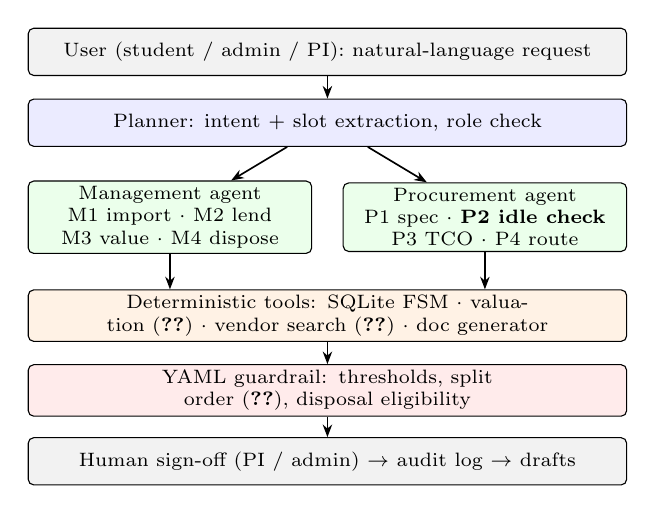
\begin{tikzpicture}[
  node distance=4mm and 3mm,
  box/.style={draw,rounded corners=2pt,align=center,font=\scriptsize,
              minimum height=6mm,inner sep=2pt},
  arr/.style={-{Stealth[length=1.6mm]},semithick}]
\node[box,fill=gray!10,minimum width=7.6cm] (user) at (0,0) {User (student / admin / PI): natural-language request};
\node[box,fill=blue!8,minimum width=7.6cm] (plan) at (0,-0.9) {Planner: intent + slot extraction, role check};
\node[box,fill=green!8,minimum width=3.6cm] (ma) at (-2.0,-2.1) {Management agent\\M1 import $\cdot$ M2 lend\\M3 value $\cdot$ M4 dispose};
\node[box,fill=green!8,minimum width=3.6cm] (pa) at (2.0,-2.1) {Procurement agent\\P1 spec $\cdot$ \textbf{P2 idle check}\\P3 TCO $\cdot$ P4 route};
\node[box,fill=orange!10,minimum width=7.6cm,text width=7.4cm] (tools) at (0,-3.35) {Deterministic tools: SQLite FSM $\cdot$ valuation (\ref{eq:value}) $\cdot$ vendor search (\ref{eq:tco}) $\cdot$ doc generator};
\node[box,fill=red!8,minimum width=7.6cm,text width=7.4cm] (guard) at (0,-4.3) {YAML guardrail: thresholds, split order (\ref{eq:split}), disposal eligibility};
\node[box,fill=gray!10,minimum width=7.6cm] (hitl) at (0,-5.2) {Human sign-off (PI / admin) $\rightarrow$ audit log $\rightarrow$ drafts};
\draw[arr] (user) -- (plan);
\draw[arr] (plan) -- (ma);
\draw[arr] (plan) -- (pa);
\draw[arr] (ma) -- (ma |- tools.north);
\draw[arr] (pa) -- (pa |- tools.north);
\draw[arr] (tools) -- (guard);
\draw[arr] (guard) -- (hitl);
\end{tikzpicture}
\caption{LabSteward architecture. Only the planner interprets language;
all values and decisions come from the lower layers.}
\label{fig:arch}
\end{figure}

% [A2Z:PH]
\textit{How the goals are met.} The idle check (P2) runs before any
vendor search and returns an internal-sharing suggestion when a matching
asset has status \texttt{IDLE} or \texttt{IN\_STOCK}. Asset states are
changed only through a finite-state machine over \{in stock, on loan,
idle, maintenance, pending disposal, disposed\}. Thresholds live in
\texttt{rules.yaml}, so a change in law needs no code change. A Streamlit
interface exposes the same loop to users.

% [A2Z:PI]
Algorithm~\ref{alg:main} gives the main loop. In the released version the
planner uses keyword and regular-expression rules; an LLM planner is a
drop-in replacement for line~1 because it only has to output the same
intent and slots.

\begin{algorithm}[t]
\caption{LabSteward main loop}
\label{alg:main}
\begin{algorithmic}[1]
\REQUIRE query $Q$, role $r$, history $H$
\STATE $(\iota,\theta)\leftarrow\textsc{Parse}(Q)$ \COMMENT{intent, slots}
\IF{$\iota\notin\textsc{Perm}(r)$} \RETURN \texttt{PERMISSION\_DENIED} \ENDIF
\IF{$\iota=$ \texttt{PROCURE}}
  \STATE $m\leftarrow\textsc{IdleMatch}(\theta.spec)$
  \IF{$m\neq\emptyset$} \RETURN \texttt{INVENTORY\_SATISFIED}$(m)$ \ENDIF
  \STATE $O\leftarrow\textsc{RankByTCO}(\textsc{Search}(\theta.spec))$
  \STATE $g\leftarrow\textsc{Guardrail}(O_1,H)$
  \IF{$g$ violated} \RETURN \texttt{GUARDRAIL\_VIOLATION} \ENDIF
\ELSE
  \STATE $res\leftarrow\textsc{Manage}(\iota,\theta)$ \COMMENT{FSM + valuation}
\ENDIF
\STATE \textsc{AuditLog}$(r,\iota,res)$; \RETURN draft for human sign-off
\end{algorithmic}
\end{algorithm}

% [A2Z:PJ]
\textit{Example.} A first-year student asks to buy an RTX~4090
workstation for 120{,}000~NTD. The planner extracts intent
\texttt{PROCURE} and the spec; P2 finds asset LAB-2024-GPU-02, an RTX~4090
workstation with 5\% utilization and status \texttt{IDLE}, and the agent
suggests an internal transfer, saving the full budget. If the student
insists, P3 ranks three vendor offers by TCO and P4 routes the
118{,}000~NTD offer to the small-purchase procedure.

% [A2Z:PK]
\textit{Key points.} (1) The idle check is structural, not advisory.
(2) Book and market values are reported together, so disposal decisions
are not driven by accounting age alone. (3) Rules are data and every
decision is logged, which makes the agent auditable.

% [A2Z:PL]
\textit{Evaluation plan.} Because every decision is deterministic, the
agent can be evaluated by executing it on scripted tasks and comparing
returned statuses with expected ones; Section~IV does this. A user study
(SUS) and the three baselines of the original plan are future steps.

% [A2Z:PM]
\textit{Safety property.} Let every state change pass through the FSM and
let the guardrail predicate $\Gamma$ be evaluated before any commit. If
retries and clarification turns are bounded by $K_{max}$ and $T_{max}$,
each query terminates in at most $K_{max}+T_{max}+c$ steps for a constant
$c$, because every step either consumes budget or moves to a terminal
state. Moreover, every committed action $a$ satisfies $\Gamma(a)$, since a
commit is reachable only through the branch where $\Gamma$ holds.
Soundness is therefore conditional on $\Gamma$ being \emph{complete}:
the proof says nothing about a rule that is missing from $\Gamma$.
Section~IV shows such a case.

% =====================================================================
\section{Experiment}
% ---------------------------------------------------------------------
% [A2Z:Q]
\textit{Metrics.} We report task success rate (returned status equals
expected status) overall and per sub-agent; pass$^4$, the share of tasks
solved in all four repeated runs~\cite{yao2024taubench}; guardrail leak
rate, the share of tasks that should be blocked but return
\texttt{SUCCESS}; duplicate-purchase rate, the share of idle-check tasks
in which the agent did not propose internal sharing; and median and
95th-percentile latency.

% [A2Z:R]
\textit{Compared methods.} We compare the released code (v1.0) with
v1.1, which applies two one-line fixes found during the measurement
(analyzed below). The original plan also lists a manual Excel workflow, a
tool-less LLM and a retrieval-only system as baselines. The earlier
evaluation script printed fixed numbers for these baselines and for
LabSteward without executing anything, so we do not report those numbers;
the baselines are \TBD.

% [A2Z:S]
\textit{Setup.} The benchmark has 50 Chinese-language tasks: 25 management
(lend, lend conflict, valuation, disposal check, disposal draft) and 25
procurement (idle pre-check, small purchase, split order, tender, vendor
quotes), five instances of each of ten templates. The inventory holds
eight seed assets. All runs use the role \texttt{pi}, Python~3.11.1 on
Windows~11, and the harness \texttt{experiments/run\_real\_eval.py}.

% [A2Z:T]
\textit{Tuned conditions.} We vary (a) the state protocol: \emph{fresh}
re-seeds the database before every task, \emph{seq} runs tasks in file
order so state carries over; and (b) the context for split-order tasks:
\emph{strict} withholds the purchase history implied by the query,
\emph{with-history} passes one earlier 80{,}000~NTD order. Valuation
parameters ($d$, $\delta$, $\alpha$) keep their released values.

% [A2Z:U]
Table~\ref{tab:results} gives the results. History made no difference in
any condition, so we show the strict runs. v1.0 solves 40.0\% of tasks in
the fresh protocol and 32.0\% in the sequential one. All failures fall
into three causes (Table~\ref{tab:fail}). (1) The document generator
formats float values with an integer format code and crashes on every
disposal path (10 tasks). (2) The disposal gate blocks only assets that
are past their statutory life and still working; LAB-2024-GPU-02 is
neither, so the gate let it through to draft generation, where cause (1)
stopped it. (3) All 20 non-idle procurement tasks return \texttt{ERROR}
because the vendor catalogue covers only two product families and the
whole sentence is passed as the specification; the split-order rule is
never reached because the guardrail runs after the search. In the
sequential protocol, the loan made by the first lend task is never
returned, so four of five later loans are correctly rejected but counted
as failures. v1.1 fixes (1) and (2), reaching 60.0\% (fresh) and 52.0\%
(seq) with 100\% management success in the fresh protocol.

\begin{table}[t]
\centering
\caption{Measured results on the 50-task benchmark (strict context).}
\label{tab:results}
\footnotesize
\begin{tabular}{lcccc}
\toprule
 & \multicolumn{2}{c}{v1.0 (released)} & \multicolumn{2}{c}{v1.1 (2 fixes)} \\
\cmidrule(lr){2-3}\cmidrule(lr){4-5}
Metric & fresh & seq & fresh & seq \\
\midrule
Success rate (\%)        & 40.0 & 32.0 & 60.0 & 52.0 \\
\quad Management (\%)    & 60.0 & 44.0 & 100.0 & 84.0 \\
\quad Procurement (\%)   & 20.0 & 20.0 & 20.0 & 20.0 \\
pass$^4$ (\%)            & 40.0 & ---  & 60.0 & --- \\
Guardrail leak (\%)      & 0.0  & 0.0  & 0.0  & 0.0 \\
Duplicate purchase (\%)  & 0.0  & 0.0  & 0.0  & 0.0 \\
Median latency (ms)      & 8.7  & 8.5  & 8.9  & 10.5 \\
\midrule
Baselines B1--B3         & \multicolumn{4}{c}{\TBD} \\
\bottomrule
\end{tabular}
\end{table}

\begin{table}[t]
\centering
\caption{Failure causes of v1.0 (fresh protocol, 30 failed tasks).}
\label{tab:fail}
\footnotesize
\begin{tabular}{p{4.6cm}cc}
\toprule
Cause & Tasks & Fixed in v1.1 \\
\midrule
Integer format code on float values in disposal draft & 10 & yes \\
Disposal gate ignores ``not yet eligible'' assets (latent leak) & 5$^{*}$ & yes \\
Vendor catalogue / spec extraction; guardrail after search & 20 & no \\
\bottomrule
\multicolumn{3}{l}{\scriptsize $^{*}$Overlaps with the first row: these 5 tasks crashed in cause~(1).}
\end{tabular}
\end{table}

% [A2Z:V]
\textit{Verification.} The results confirm two claims and correct
others. Confirmed: the idle-inventory check proposed internal sharing in
5 of 5 idle-check tasks in every condition, and no task that should be
blocked returned \texttt{SUCCESS}; decisions are reproducible, so
pass$^4$ equals the success rate, which avoids the consistency problem of
LLM agents~\cite{yao2024taubench}. Corrected: the overall success rate is
far below the 96\% printed by the earlier script, and the zero leak rate
in v1.0 was partly luck, because cause (2) is a missing rule that the
safety argument of Section~III cannot detect. The measurement also has
limits: the 50 tasks contain only ten distinct templates, latency excludes
any LLM call, and baselines are not yet implemented.

% =====================================================================
\section{Conclusion}
% ---------------------------------------------------------------------
% [A2Z:W]
We set out to reduce idle laboratory equipment and rule violations in
university purchasing, where existing systems record ownership but not
use, and where LLM agents are unstable and unaware of procurement law.

% [A2Z:X]
LabSteward is strongest where the decision is rule-bound: it makes the
idle-inventory check a mandatory step, keeps every number and threshold
in deterministic tools and a YAML rule file, and reports book and market
value side by side.

% [A2Z:Y]
On the measured 50-task benchmark, the released version solved 40.0\% of
tasks and the fixed version 60.0\%, with 100\% management success,
5-of-5 idle detection and no leaked violations. Procurement success stays
at 20.0\% because of catalogue coverage and the guardrail order.

% [A2Z:Z]
The main lesson is that executing the agent, rather than printing
expected numbers, found two defects in a single run, and that a safety
proof only covers the rules that were written down. Next we will run the
guardrail before vendor search, replace keyword extraction with an LLM
planner, expose the tools through MCP~\cite{mcp2024}, add the three
baselines and more diverse tasks, and conduct a user study.

% =====================================================================
\begin{thebibliography}{00}
\bibitem{yao2023react} S.~Yao, J.~Zhao, D.~Yu, N.~Du, I.~Shafran, K.~Narasimhan, and Y.~Cao, ``ReAct: Synergizing reasoning and acting in language models,'' in \textit{Proc. ICLR}, 2023.
\bibitem{yao2024taubench} S.~Yao, N.~Shinn, P.~Razavi, and K.~Narasimhan, ``$\tau$-bench: A benchmark for tool-agent-user interaction in real-world domains,'' arXiv:2406.12045, 2024.
\bibitem{lyu2025deepshop} Y.~Lyu \textit{et al.}, ``DeepShop: A benchmark for deep research shopping agents,'' arXiv:2506.02839, 2025.
\bibitem{peeters2025entity} R.~Peeters, A.~Steiner, and C.~Bizer, ``Entity matching using large language models,'' in \textit{Proc. EDBT}, 2025.
\bibitem{singh2025agenticrag} A.~Singh, A.~Ehtesham, S.~Kumar, and T.~Talaei~Khoei, ``Agentic retrieval-augmented generation: A survey on agentic RAG,'' arXiv:2501.09136, 2025.
\bibitem{duan2025askclarify} Y.~Duan, Y.~Hu, and J.~Jiang, ``Ask, clarify, optimize: Human-LLM agent collaboration for smarter inventory control,'' arXiv:2601.00121, 2025.
\bibitem{huymajer2025residual} M.~Huymajer, P.~Filzmoser, A.~Mazak-Huemer \textit{et al.}, ``Opportunities and pitfalls of regression algorithms for predicting the residual value of heavy equipment,'' \textit{Eng. Appl. Artif. Intell.}, vol.~141, p.~109599, 2025.
\bibitem{reznicek_price} T.~\v{R}ezn\'{i}\v{c}ek and T.~Krop\'{i}k, ``The effect of age and selected characteristics on the asking price of movable property,'' n.d.
\bibitem{schick2023toolformer} T.~Schick \textit{et al.}, ``Toolformer: Language models can teach themselves to use tools,'' in \textit{Proc. NeurIPS}, 2023.
\bibitem{controlyuan2013} Control Yuan (Taiwan), ``Investigation report on valuable instruments funded by the National Science Council,'' 2013.
\bibitem{gpa_tw} Public Construction Commission, Executive Yuan (Taiwan), ``Government Procurement Act,'' Art.~14 and threshold regulations.
\bibitem{mcp2024} Anthropic, ``Model Context Protocol specification,'' 2024. [Online]. Available: \url{https://modelcontextprotocol.io}
\end{thebibliography}

\end{document}
